\documentclass{scrreprt}

\usepackage{graphicx}
\usepackage{tikz}
\usepackage{amstext}
\usepackage{hyperref}
\usepackage{amsfonts}
\usepackage{tabularx}
\usepackage{multirow}
\usepackage{amssymb}
\usepackage{textcomp}
\usepackage[left=2.5cm, right=2.5cm, top=2cm, bottom=2cm]{geometry}
\newcommand\tab[1][1cm]{\hspace*{#1}}

\usepackage{listings}
\usepackage{color}

\definecolor{dkgreen}{rgb}{0,0.6,0}
\definecolor{gray}{rgb}{0.5,0.5,0.5}
\definecolor{mauve}{rgb}{0.58,0,0.82}

\lstset{frame=tb,
  language=Java,
  aboveskip=3mm,
  belowskip=3mm,
  showstringspaces=false,
  columns=flexible,
  basicstyle={\small\ttfamily},
  numbers=none,
  numberstyle=\tiny\color{gray},
  keywordstyle=\color{blue},
  commentstyle=\color{dkgreen},
  stringstyle=\color{mauve},
  breaklines=true,
  breakatwhitespace=true,
  tabsize=3
}

\hypersetup{
  colorlinks=false,
  linkbordercolor=blue,
  pdfborderstyle={/S/U/W 0}
}
\title{\textbf{Algorithmen und Datenstrukturen}}
\author{\href{https://github.com/bircni}{\color{blue}github/bircni}}
%\date{\href{https://ko-fi.com/toiletcoders}{\color{black}little donation}}
\begin{document}
\pagenumbering{gobble}
\maketitle
\pagebreak
\renewcommand{\contentsname}{Inhaltsverzeichnis}
%\renewcommand{\cftdot}{}
\setcounter{tocdepth}{1}
\tableofcontents
\addtocontents{toc}{~\hfill\textbf{Seite}\par}
\pagebreak
%\pagenumbering{arabic}
\chapter{Mathematische Grundlagen}
\section{Reihen}
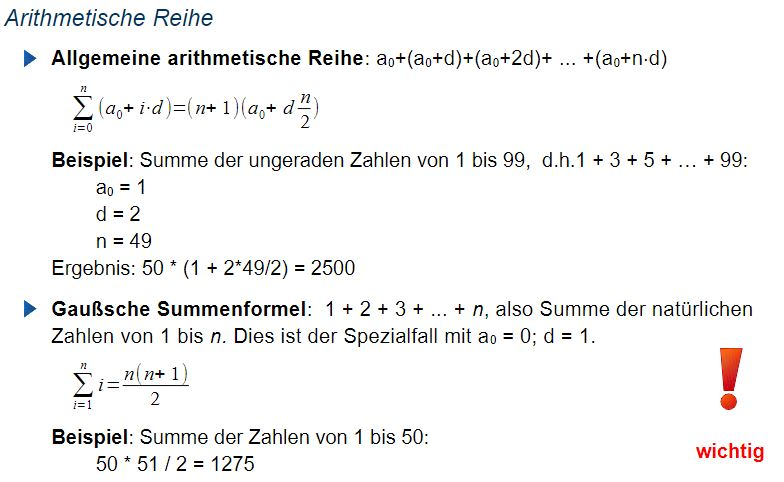
\includegraphics[width=0.65\textwidth]{graphics/reihen-arithmetisch}
\section{Potenzen und Logarithmen}
Der Logarithmus ist die Inverse der Potenzfunktion. $\log_a(x) = y \quad \Longleftrightarrow  \quad a^y = x$
\\\textbf{spezielle Logarithmen:}
\\$ld(x)=log_2(x)$, $lg(x)=log_10(x)$, $ln(x)=log_e(x)$
\section{Notationskonventionen}
$\lceil x \rceil$ zur nächsten ganzen Zahl aufrunden
\\$\lfloor x \rfloor$ zur nächsten ganzen Zahl abrunden
\\$[a .. b] = {x \arrowvert a \leq x \wedge x \leq b}$ mit Intervallgrenzen
\\$]a .. b[ = {x \arrowvert a < x \wedge x < b}$ ohne Intervallgrenzen
\\$arr[i .. k]$ Teilfolge der Elemente von $arr[i]$ bis $arr[k]$
\section{Grundbegriffe der Graphentheorie}
Graphen bestehen aus einer Menge von Knoten und Kanten, die diese verbinden.
\\Ein Graph ist gerichtet, wenn die Kanten eine Richtung haben.
\\Für einen Knoten v eines gerichteten Graphen $G=(V,E)$ ist der Eingangsgrad $indeg(v)$ die Anzahl der Kanten,
die in v enden, und der Ausgangsgrad $outdeg(v)$ die Anzahl der Kanten, die von v ausgehen.
\\Ein Zyklus ist ein Weg der bei einem Knoten startet und endet.
\\Ein gerichteter Graph ist zusammenhängend, wenn es einen Weg zwischen jedem Knotenpaar gibt.
\\Ein Baum hat einen Knoten als Wurzel, jeder Knoten hat genau einen Vorgänger und ist zusammenhängend.
\\Ein Knoten ohne Kinder heißt Blatt. Ein leerer Baum hat die Höhe 0.
Ein Binärbaum ist ein Baum, dessen Knoten maximal zwei Kinder haben.
\\Traversierungen: Preorder (WLR), Inorder (LWR), Postorder (LRW)
\chapter{Rekursive Algorithmen}
\section{Prinzip der Rekursion}
Ein rekursiver Algorithmus besteht aus einem Basisfall und einem rekursiven Aufruf.
\\Der rekursive Aufruf muss immer kleiner werden, damit die Rekursion endet.
\\Die Rekursion kann durch eine Schleife ersetzt werden.
\begin{lstlisting}
  public static double sum_v2(double[] arr) {
  return sum_v2(arr, 0, arr.length-1);
  }
/** Berechnet Summe der Werte von arr[firstIndex..lastIndex] */
  private static double sum_v2(double[] arr, int firstIndex,int lastIndex) {
  if (firstIndex == lastIndex) {
    // zu summierender Bereich besteht nur aus einem Element
    return arr[firstIndex];
  }
  else {
    int mid = (firstIndex + lastIndex) / 2;
    return sum_v2(arr, firstIndex, mid) + sum_v2(arr, mid+1, lastIndex);
  }}
  \end{lstlisting}
\section{Korrektheit rekursiver Algorithmen}
Ein Beweisverfahren ist die Berechnungsinduktion.
\\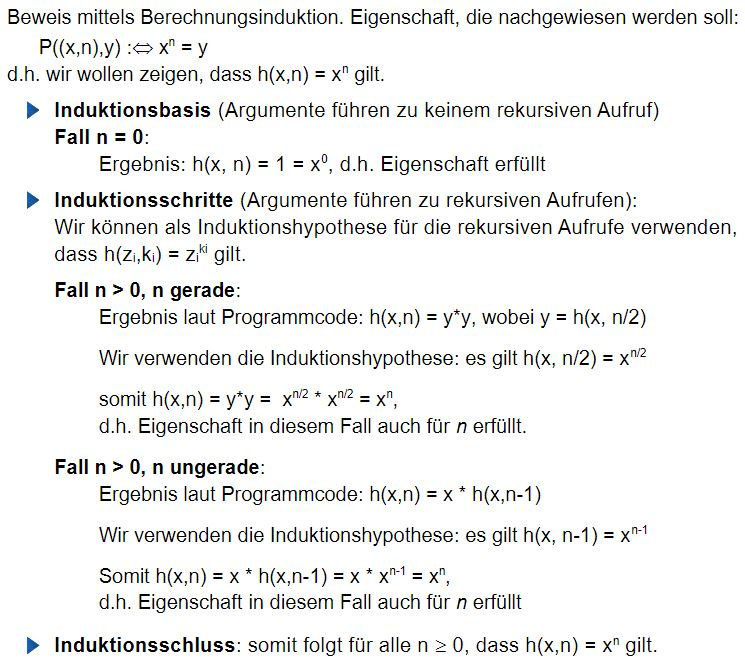
\includegraphics[width=0.8\textwidth]{graphics/3-2Korrektheit}
\section{Rekursive Berechnung der Potenzmenge}
\textbf{Beispiel:}
\\Menge: $M =\{a,b,c\}$
\\Potenzmenge: $\rho (M) = \{ \emptyset, \{a\}, \{b\}, \{c\}, \{a,b\}, \{a,c\}, \{b,c\}, \{a,b,c\} \}$
\subsection{Rekursiver Lösungsansatz}
a) in welchen einfach Fällen kann die Lösung direkt angegeben werden?
\\\tab der einfachste Fall ist die leere Menge $M = \emptyset$
\\\tab die leere Menge hat nur sich als Teilmenge $\rho(\emptyset) = \{\emptyset\}$
\\b) Wie können in nicht einfachen Fällen die Teilmengen bestimmt werden?
\\\tab Sei Menge $M = \{a_1,\ldots,a_{n-1},a_n\}$ nicht leer $(n\geq1)$
\begin{itemize}
  \item [1.] Wir wählen ein Element der Menge, z.B. $a_n$
  \item [2.] Es gibt nun zwei Arten von Teilmengen:
  \begin{itemize}
    \item [$T^+$] Teilmengen, die das Element $a_n$ enthalten
    \item [$T^-$] Teilmengen, die das Element $a_n$ nicht enthalten
  \end{itemize}
  Die Menge aller Teilmengen ist die Vereinigung von $T^+$ und $T^-$, d.h. $\rho(M) = T^+ \cup T^-$
  \\Die Menge $T^+$ kann nun rekursiv berechnet werden, indem wir $a_n$ aus $M$ entfernen und die Potenzmenge von $M$ berechnen.
  \\Die Menge $T^-$ ist die Potenzmenge von $M$ ohne $a_n$.
  \\Die Potenzmenge von $M$ ist also die Vereinigung von $T^+$ und $T^-$.
\end{itemize}
\textbf{Beispiel:} Wenn $M = \{a,b,c\}$
\\\tab Wähle z.B. c als Element:
\\\tab $T^-$: alle Teilmengen ohne c, also alle Teilmengen von $\{a,b\}$
\\\tab\tab $T^- =\{\emptyset,\{a\},\{b\},\{a,b\}\}$
\\\tab $T^+$: alle Teilmengen mit c, Nimm zu jeder Teilmenge von $T^-$ und füge c hinzu
\\\tab\tab $T^+ = \{\{c\},\{a,c\},\{b,c\},\{a,b,c\}\}$
\\\tab Insgesamt: $\rho(\{M\}) = T^+ \cup T^- =\{\emptyset,\{a\},\{b\},\{a,b\},\{c\},\{a,c\},\{b,c\},\{a,b,c\}\}$
\subsection{Algorithmischer Ansatz}
\textbf{Falls M leer} ($M = \emptyset$)
\\\tab leere Menge ist die einzige Teilmenge
\\\textbf{Falls M nicht leer} Wähle ein Element $a_n$ aus $M$
\\\tab Berechne Sammlung $T^-$ aller Teilmengen von M ohne $a_n$ (rekursiv)
\\\tab Berechne Sammlung $T^+$ aller Teilmengen, die $a_n$ enthalten:
\\\tab Nimm dazu jede Menge aus $T^-$ und bilde eine neue Menge, indem $a_n$ hinzugefügt wird
\\\tab Die Menge aller Teilmengen ist die Vereinigung von $T^+$ und $T^-$
\\\begin{lstlisting}
private static <E> Set<Set<E>> allSubsets(E[] arr,int maxIndex) {
Set<Set<E>> resultSet = new HashSet<Set<E>>();
if (maxIndex >= 0) {
  // Menge ist nicht leer, waehle letzes Element im gegebenen Bereich
E selected = arr[maxIndex];
  // Bilde rekursive alle Teilmengen ohne selected
Set<Set<E>> resultSet1 = allSubsets(arr, maxIndex - 1);
  // nimm jede dieser Mengen zum Ergebnis hinzu
resultSet.addAll(resultSet1);
  // bilde alle Teilmengen, die selected enthalten
for (Set<E> set1 : resultSet1) {
  // Erzeuge Kopie der Menge aus resultSet1 und nimm gewaehltes Element dazu
Set<E> set2 = new HashSet<E>(set1);
set2.add(selected);
  // fuege die ergaenzte Kopie zum Ergebnis hinzu
resultSet.add(set2);
}
} else {
  // Menge ist leer. Leere Menge hat nur leere Menge als einzige Teilmenge
Set<E> emptySet = new HashSet<>();
resultSet.add(emptySet);
}
return resultSet;
}
\end{lstlisting}
\section{Algorithmenprinzip ''Backtracking''}
\subsection{Grundidee ''Trial and Error''} 
\begin{itemize}
  \item [1.] Versuche eine Lösung zu finden
  \item [2.] Wenn die Lösung nicht passt, versuche eine andere Lösung
  \item [3.] Wenn keine Lösung passt, gehe zurück und versuche eine andere Lösung
\end{itemize}

\chapter{Analyse von Algorithmen}
\section{Korrektheit}
\subsection{Insertionsort}
\begin{itemize}
  \item Am Anfang des Arrays wird ein sortierter Bereich aufgebaut, in den nach und nach die folgenden Elemente 
  eingefügt werden (deshalb ''Insertionsort'').
  \item Am Anfang besteh der sortierte Bereich nur aus dem ersten Element $arr[0]$.
  \item In jedem Schritt wird ein Element $arr[i]$ aus dem unsortierten Bereich in den sortierten Bereich eingefügt.
  \item Wenn alle Elemente eingefügt wurden, ist das Array sortiert.
\end{itemize}
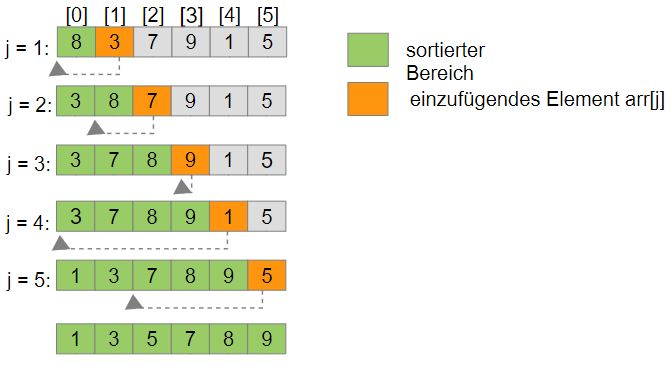
\includegraphics[width=0.65\textwidth]{graphics/insertionsort}
\\\textbf{Definition:}
\\ Enthält ein Array arr am Anfang die n Elemente $arr[0],arr[1],\dots,arr[n-1]$, so ist das Array sortiert, wenn gilt:
\begin{itemize}
  \item \textbf{Permutationen:} Die Elemente von arr sind eine Permutattion (Umordnung) der ursprünglichen 
  Elemente von $[0,n-1]$.
  \item \textbf{Monotonie:} Die Elemente von arr sind monoton steigend/fallend sortiert.
\end{itemize}
Mit \textbf{sortiert} ist sofern nicht anders angegeben immer \textbf{aufsteigend sortiert} gemeint.
\section{Komplexität von Algorithmen}
Komplexität bezeichnet den Ressourcenverbrauch von Algorithmen. Ressourcen sind dabei die Ausführungszeit und der Speicherbedarf.
\\Der Ressourcenbedarf hängt von mehreren Faktoren ab:
\begin{itemize}
  \item Umfang der Daten (Größe des Problems)
  \item Zusammensetzung der Daten (aktuelle Sortierung der Daten)
  \item Ausführungsgeschwindigkeit und Speicherbedarf bei der Ausführung
\end{itemize}
\subsection{Vorgehen bei der Laufzeitanalyse}
\begin{itemize}
  \item Bestimme für jede Anweisung $A_j$ des Programms die Häufigkeit $k_j$ der Ausführung.
  \item Die Gesamtkosten bei Problemgröße $n$ können dann so zusammengezählt werden:
  $T(n) = \sum_{A_j}^n k_j \cdot c_j$
  \\wobei $k_j$ die Häufigkeit für die Ausführung von Anweisung $A_j$ ist
  \\und $c_j$ die Einzel-Ausführungszeit für $A_j$ ist.
\end{itemize}
\subsection{Abhängigkeit von der Datenzusammensetzung}
\textbf{Best Case:} basiert auf Daten, die im Algorithmus eine minimale Anzahl von Schritten erfordern.
\\\textbf{Worst Case:} basiert auf Daten, die im Algorithmus eine maximale Anzahl von Schritten erfordern.
\\\textbf{Average Case:} basiert auf Daten, die im Algorithmus eine durchschnittliche Anzahl von Schritten erfordern.
\\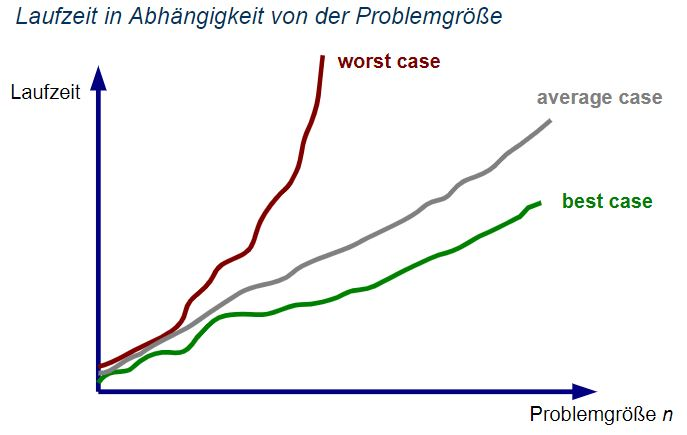
\includegraphics[width=0.65\textwidth]{graphics/Laufzeit}
\subsection{Häufig verwendete Größenordnungen}
\begin{itemize}
  \item $O (1)$: Konstante Laufzeit - elementare Operationen
  \item $O (\log n)$: Logarithmische Laufzeit - binäre Suche
  \item $O (n)$: Lineare Laufzeit - lineare Suche
  \item $O (n \log n)$: Logarithmische Laufzeit - schnelle Sortieralgorithmen
  \item $O (n^2)$: Quadratische Laufzeit - einfache Sortieralgorithmen
  \item $O (n^3)$: Kubische Laufzeit
  \item $O (c^n)$: Exponentielle Laufzeit
  \item $O (n!)$: Permutationen berechnen
\end{itemize}
\section{Komplexitätsanalyse wohlstrukturierter Algorithmen}
Unter wohlstrukturierten Algorithmen versteht man solche, die nur mit Hilfe von Sequenz (nacheinander ausführen),
Alternative (Fallunterscheidung) und Iteration (Schleife) definiert sind.
\subsection{Lineare Suche}
Bei der linearen Suche wird ein Array von links nach rechts durchsucht, bis das gesuchte Element gefunden wurde.
\\\begin{lstlisting}[language=Java]
public String sucheNummer(String suchname) {
  for (int i = 0; i < anzahl; i++) {
    if (liste[i].name.equals(suchname))
    return liste[i].nummer;} // gefunden
return null;} // nicht gefunden
\end{lstlisting}
\subsection{Binäre Suche}
Bei sortierten Daten kann der Bereich, in dem der gesuchte Schlüssel liegen kann, nach und nach immer wieder 
halbiert werden. Dieses Verfahren wird \textbf{binäre Suche} genannt.
\\\begin{lstlisting}[language=Java]
private String searchBinRek(String sname, int from, int to){
  if (to < from) {
    return null; //leerer Suchbereich, nichts gefunden
  } else {
  // Mitte des Suchbereichs berechnen
  int middle = (from + to) / 2;
  // Element in der Mitte vergleichen
  int res = suchname.compareTo(liste[middle].name);
    if (res < 0) {
    // in unterer Haelfte weitersuchen
    return searchBinRek(sname, from, middle-1);
    } else if (res > 0) {
    // in oberer Haelfte weitersuchen
    return searchBinRek(sname, middle+1, to);
    } else // (res == 0) {
    // Schluessel gefunden
  return liste[middle].number;
}}}
\end{lstlisting}

\chapter{Sortierverfahren}
\section{Vergleichsbasierte Sortierverfahren}
\textbf{Interne und Externe Sortierverfahren}
\begin{itemize}
  \item \textbf{Interne Sortierverfahren:} alle Datensätze passen in den Hauptspeicher.
  \item \textbf{Externe Sortierverfahren:} nur ein Teil der Datensätze passt in den Hauptspeicher.
\end{itemize}
Eine Ordnungsrelation heißt \textbf{total} wenn sie
\begin{itemize}
  \item die Eigenschaften einer Halbordnung erfüllt (reflexiv, transitiv, antisymmetrisch)
  \begin{itemize}
    \item reflexiv: $a \leq a$
    \item transitiv: $a \leq b$ und $b \leq c$ $\Rightarrow$ $a \leq c$
    \item antisymmetrisch: $a \leq b$ und $b \leq a$ $\Rightarrow$ $a = b$
  \end{itemize}
  \item und alle Werte miteinander vergleichbar sind.
\end{itemize}
\textbf{Vergleiche über Interface Comparable}
\begin{lstlisting}[language=Java]
public interface Comparable {
  int compareTo(Object o) throws ClassCastException;
}
\end{lstlisting}
wenn $x < y$ dann $x.compareTo(y) < 0$
\\wenn $x = y$ dann $x.compareTo(y) = 0$
\\wenn $x > y$ dann $x.compareTo(y) > 0$
\subsection{Laufzeitkomplexität von Selection-Sort}
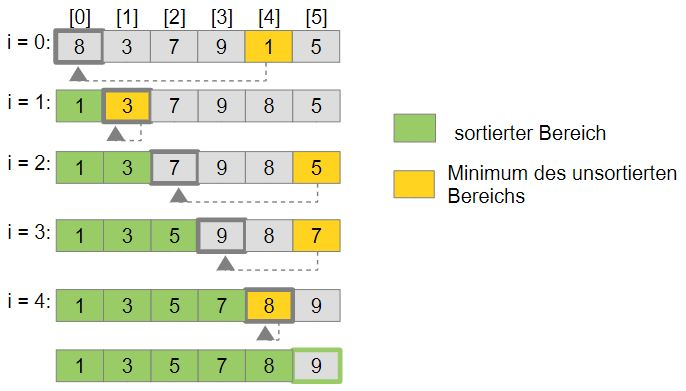
\includegraphics[width=0.65\textwidth]{graphics/Selectionsort}
\\\textbf{Worst Case = Best Case = Average Case:} $O(n^2)$
\subsection{Laufzeitkomplexität von Bubble-Sort}
\textbf{Best Case:} $O(n)$ - Daten sind schon aufsteigend sortiert
\\\textbf{Worst Case:} $O(n^2)$ - Daten sind absteigend sortiert
\\\textbf{Average Case:} $O(n^2)$
%start Lektion Nr8
\end{document}